\section{Brick Manufacturing Process}
% Information about the manufacturing process of bricks.

\subsection{Block Diagram}
% Description of the block diagram of the brick manufacturing process.
\begin{figure}[h]
  \centering
  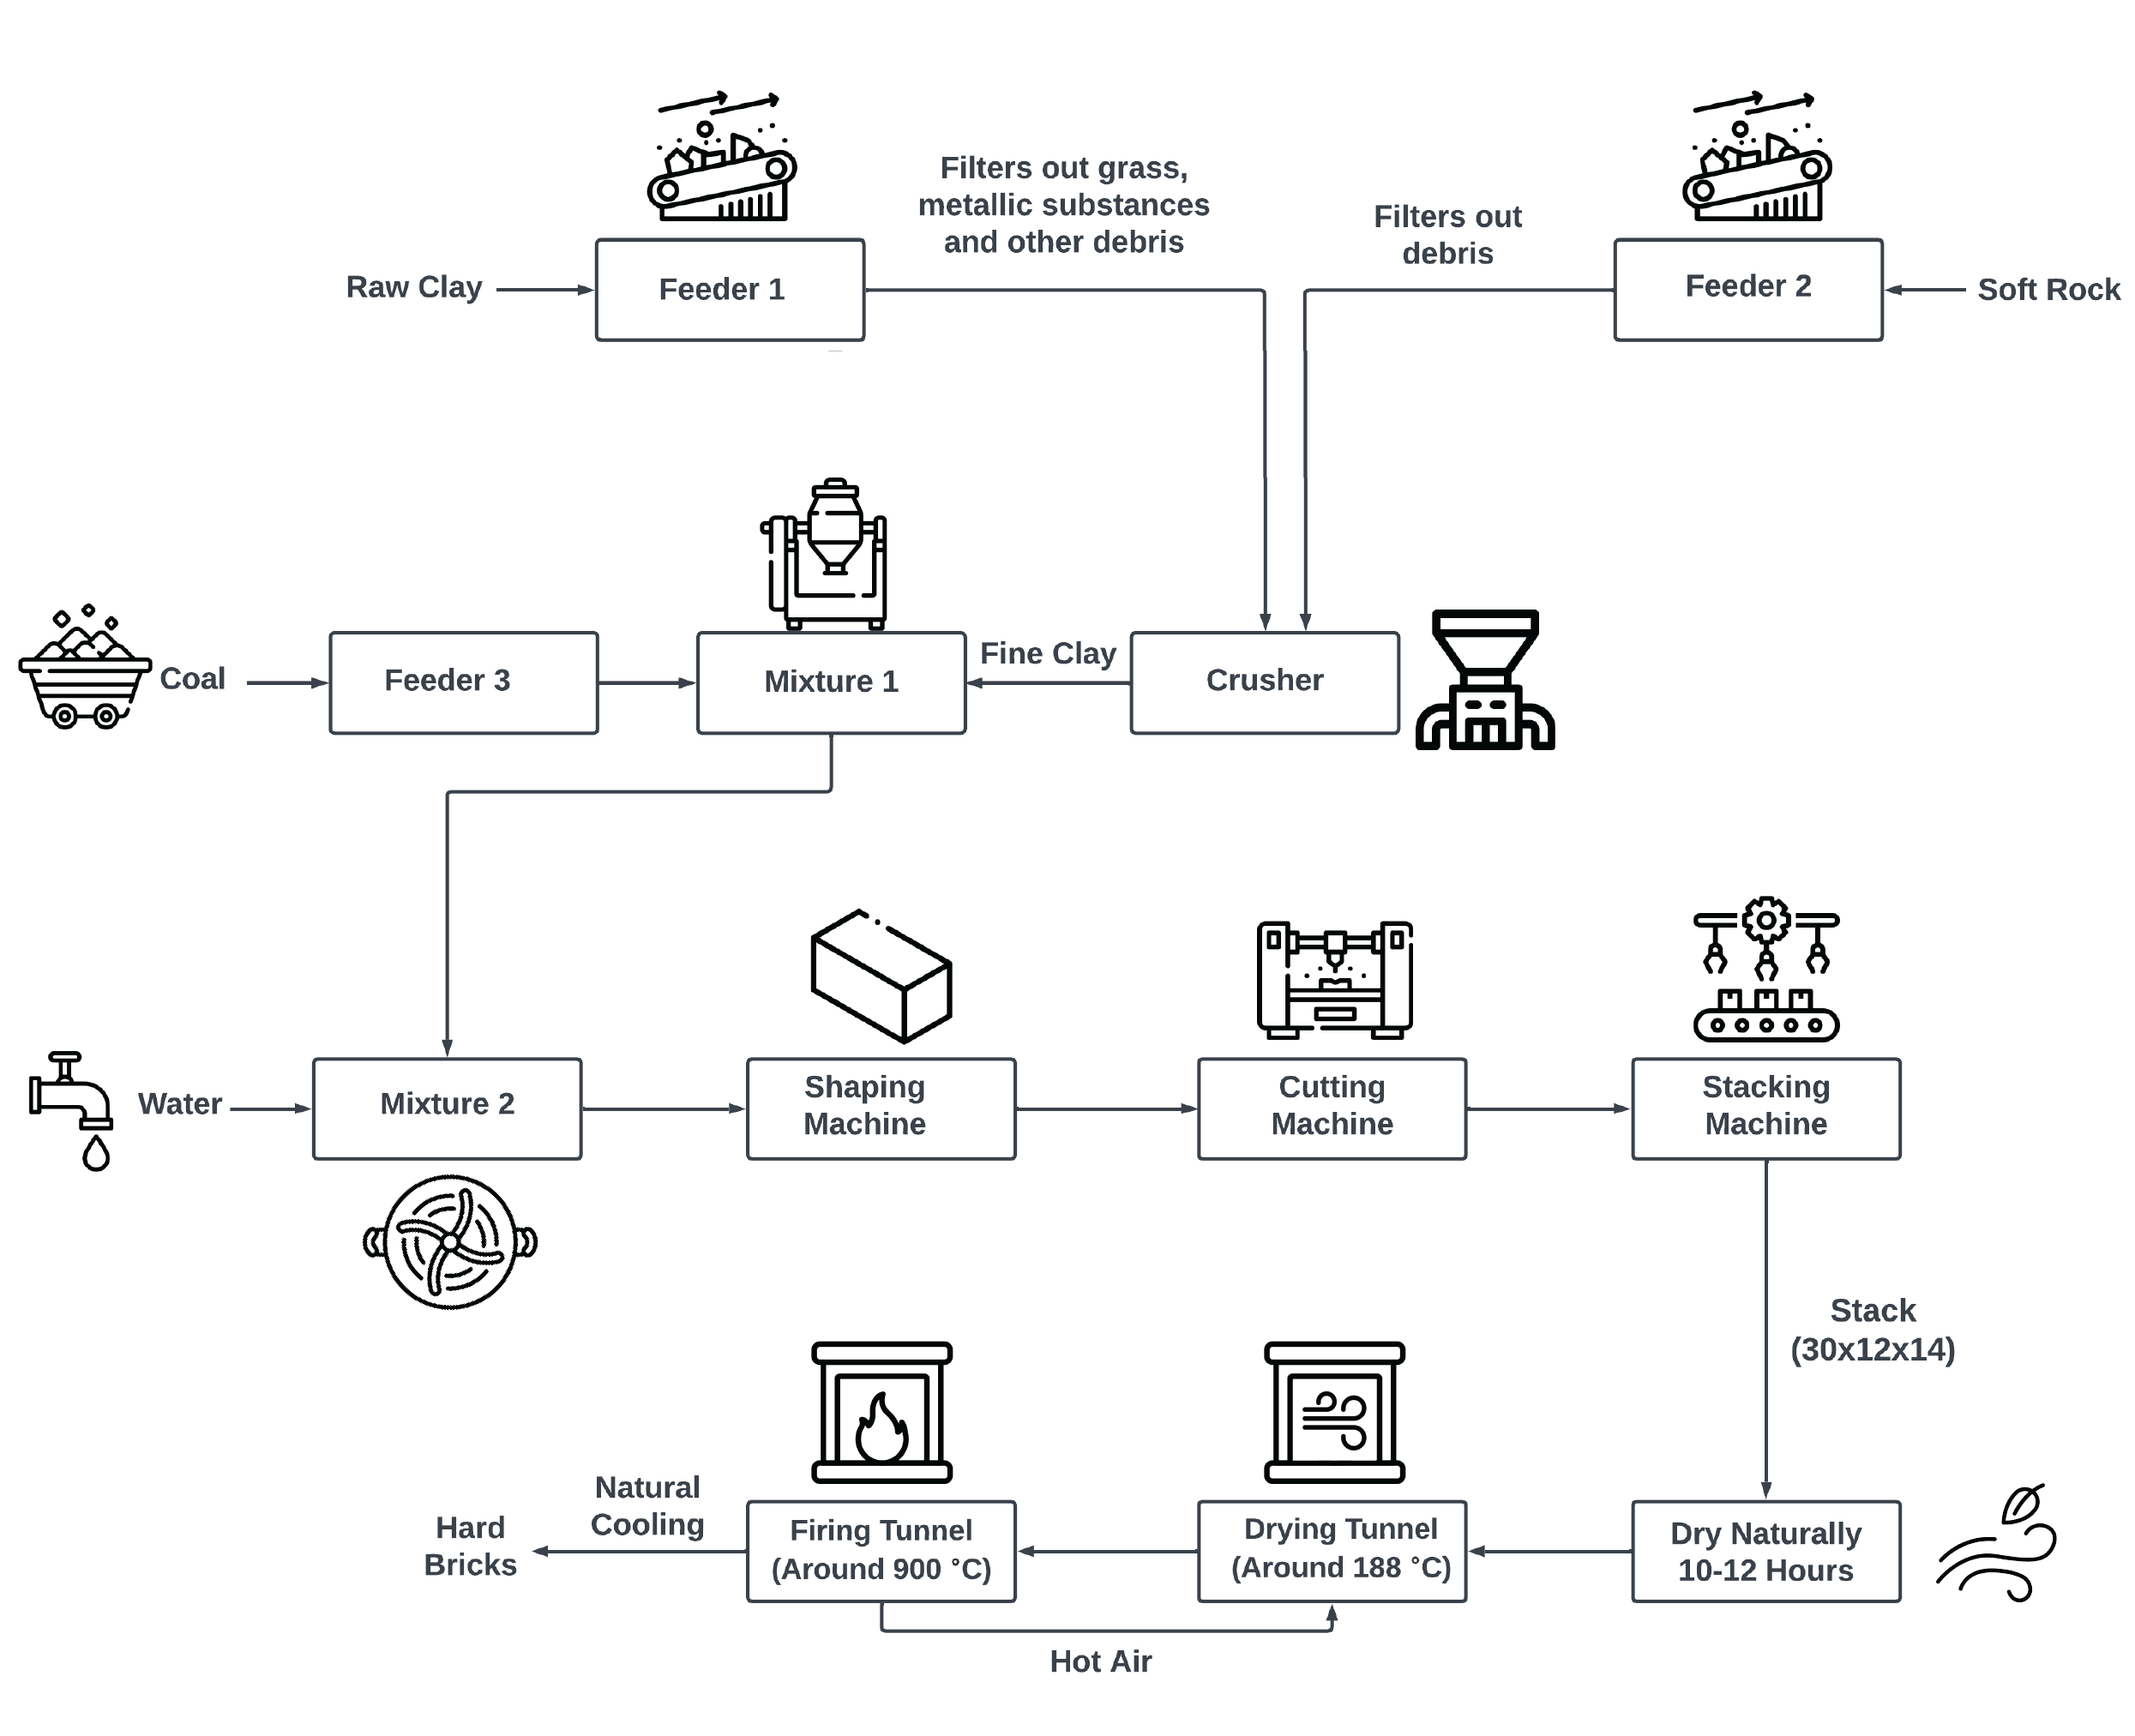
\includegraphics[width=1\textwidth]{img/block diagram.png}
  \caption{Block diagram for brick manufacture process}
\end{figure}

\subsection{Process Flow for Brick Manufacture}
Following are the basic steps of manufacturing bricks:
\begin{enumerate}
\item Clay Preparation
\item Compact Formation
\item Drying
\item Kiln Firing
\item Gradual Cooling
\end{enumerate}

\newpage

\subsection*{Clay Processing}
First, large chunks of clay are strained using a big strainer. This strainer breaks down the big chunks into smaller pieces. These smaller pieces then pass through a feeder machine. The clay is moved along a rubber conveyor belt to filter out things like grass and unwanted debris. On different parts of the rubber conveyor belt, there are strong magnets placed above to remove any metal from the clay.

Once the clay is roughly filtered, a suitable amount of soft rocks is added to it. The mixture goes through another filtering process. After the filtering is good enough, the mixture is further processed by hammering and thorough mixing to create a finer blend. A small amount of coal is mixed into this fine mixture. This mixture then goes through another feeder, entering mixing machines. Multiple mixing machines ensure proper blending of the clay. Water is also added to the clay in these machines to create a dough-like mixture.

\subsection*{Compact Formation}
The compact form of clay, molded into brick-like shapes, is known as a "cake." This cake is a vital starting point in the brick-making process. The clay, resembling dough in its texture, is carefully fed through a machine that works to create a consistent and tightly packed structure of clay. This process ensures that the clay is ready for the next steps.

Following this preparation, the clay goes through a precision-cutting phase utilizing a pressure wire cutter. This step results in the clay being divided into smaller lengths, setting the stage for the formation of individual bricks. Each length of clay, once cut by this machine, yields approximately 8 separate bricks.

As these batches of bricks take shape, a specialized mechanism steps in to lift and position them onto a waiting cart. Each cart is made to carry a good number of bricks, fitting in dimensions of about 30 by 12 by 14. The bricks are stacked alternatively to ensure stability. These carts, filled with bricks ready for further processing, are then set into motion by automated machinery.

\subsection*{Drying}